\documentclass[conference]{IEEEtran}
\IEEEoverridecommandlockouts
\usepackage{cite}
\usepackage{amsmath,amssymb,amsfonts}
\usepackage{algorithmic}
\usepackage{graphicx}
\usepackage{textcomp}
\usepackage{hyperref}
\usepackage{xcolor}
\begin{document}
\title{Study on Factors Affecting Country's Growth}

\author{\IEEEauthorblockN{1\textsuperscript{st} Neeraj Gopalakrishnan}
    \IEEEauthorblockA{\textit{Computer Science and Engineering} \\
        \textit{PES University}\\
        Bangalore, India \\
        neerajperso@gmail.com}
    \and
    \IEEEauthorblockN{2\textsuperscript{nd} Hritik Sharma}
    \IEEEauthorblockA{\textit{Computer Science and Engineering} \\
        \textit{PES University}\\
        Bangalore, India \\
        hritiks2012@gmail.com}
    \and
    \IEEEauthorblockN{3\textsuperscript{rd} Priya Gawli}
    \IEEEauthorblockA{\textit{Computer Science and Engineering} \\
        \textit{PES University}\\
        Bangalore, India \\
        priyagawli99@gmail.com}

}

\maketitle
\begin{abstract}
    The goal of this project is to create a basis of analysis that corroborates the relation between factors that affect a country's economy.\\
    In the first stage of this report, we wish to demonstrate the synopsis of the problem statement, explain the data and it's relation using an Exploratory data analysis(EDA]. The problem statement is explored from various angles using other existing papers and kaggle EDAs.\\
    The plan moving further will be to perform a few more EDA/Visualization to further our understand of the dataset and clean to improve the model to be more forgiving and informative for a larger scope of analysis. This will help the model forcast with an even higher accuracy. We also plan to experiment with various models in order to select the most optimal one.
\end{abstract}
\bigskip
\begin{IEEEkeywords}
    Prediction/Forecasting, Macroeconomies, Global Goals(UN's), Multiple Linear regression, Time-Series Analysis
\end{IEEEkeywords}
\section{Introduction}
The economic growth of the country is what defines the countrys development rate in a global scale.
But as the time passes by and the way the goals are aligned to be a more stable economy or the gloabal goal of
being more suststainable has become a primary focus than a higher economic power,
and the means to forecast the growth of the economy becomes more complicated.\\
Almost all of the country's problems can be analysed with the context of its economic growth.

This economic growth has various factors that influence it's trend; some obvious ones like: Gross-Domestic-Procduct(GDP) per Capita, Unemployment rate, Population Growth, Government Expenditure, etc; and some not so obvious ones like: Firms with female ownership, Lending interest rate, etc.
Other than these convential metrics for measuring growth we have:\\
\begin{itemize}
    \item The Impact of Human Resources
    \item Investment of capital
    \item Availability of Natural Resources
    \item Improvement in Technology
\end{itemize}
\bigskip
For our project we will be estimating the GDP on-a-country-basis which will help us project or forecast where the countries GDP might be in the forecoming future.
GDP measures the monetary value of final goods and services—that is, those that are bought by the final user—produced in a country in a given period of time (say a quarter or a year).
It counts all of the output generated within the borders of a country.
GDP is composed of goods and services produced for sale in the country, not only that but also includes some non-market related products sales and it's production, such as defense or education services provided by the government.
An alternative concept, gross national product, or GNP, counts all the output of the residents of a country.
\\
But nowadays since the global goals of UN for countries is to target a sustainable goal development it is necessary for newer alternatives that is subjected to more scrutiny for even the macro factors such as waste produced per capita gained to see if that portion of economic growth is sustainable or not.
\\The goal of our project is to quatify GDP as a factor of growth and be able to estimate how the trends for the future of the economy would be. It focuses more on growth than sustainable development, but we will look into the factors that affect the "Sustainable Development Goals" too
\bigskip
\section{Literature Review}
\emph{A. How big of an impact does expenditure on health care have on GDP?}
\\The study of this research paper attempt to identify an association of the life expectancy with healthcare expenditure and GDP in Bangladesh. The researchers of this study generate the analysis to look for an association of GDP with government funding towards health care sector and life expectancy.
Their study details about the total government spending on heatlth-care as their national expenditure and is calculated as a share of GDP, which can vary according to the country's priorities which it can be contingent on the capacity to pay and fiscal(budgetory) restraints of a fiscal year. Also, the fact that government funding towards healthcare sector is biased based on aspects like distribution of young-older population, urban-to-rural ratios, and burden of contagious and the non-spreading diseases reflects also on the amount of money needed for the healthcare of the country. However, life expectancy is also unequally distributed globally. For example, life expectancy is often better in the developed countries, as compared to that of the developing countries.
\\For the study, they collected total health expenditure and GDP for the year of 1996 to 2006 from “Bangladesh Health Bulletin 2011” and the life expectancy for the same period was taken from “Sample Vital Registration System 2010” respectively. To compare life expectancy with the total health expenditure, fiscal year has been considered. Total health expenditure and GDP were expressed using both the Bangladeshi taka (BDT) and USD [Dollars].
\\Total health expenditure includes all of the payments like spending for doctor's consultation fees, medication, laboratory tests and hospital bills. Here the term life expectancy means an expectation of longevity i.e. expected years for a person to survive. They considered Total Health Expenditure (THE) as dependent variable and independent variables are life expectancy and GDP. They performed the analysis using STATA version 13 SE (College Station, Texas, USA). Graphical presentation and descriptive statistics were performed to present the findings. Multivariate logistic regression was carried out to find the association of total health expenditure with life expectancy and fig1. total health expenditure, GDP and Life expectancy from 1997 to 2007 in Bangladesh. GDP. A conventional cut-off value of 0.05 was taken as statistical significance.
\\From this study, they found a direct relationship of total health expenditure and life expectancy in bi-variable analysis.
\begin{figure}[htbp]
    \centerline{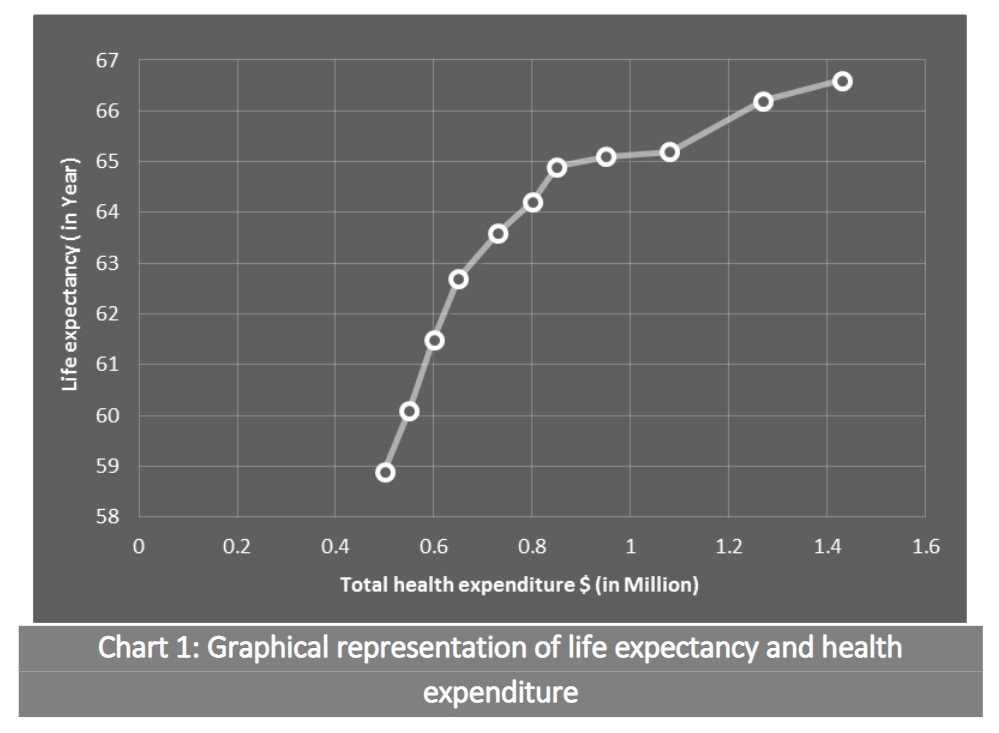
\includegraphics[scale=0.5]{healthcare1.jpg}}
    \caption{Graphical representation of life expectancy and health expenditure}
\end{figure}
\\A priori was considered expecting that both the GDP and LE will have a positive impact on THE. Thus their proposed econometric model is-
\begin{figure}[htbp]
    \centerline{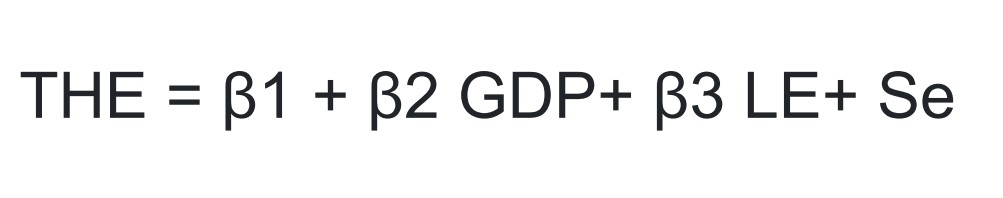
\includegraphics[scale=0.3]{healthcare3.jpg}}
    \caption{Formulae 1.1}
\end{figure}
\\As in Fig.3, Beta1 is the intercept and Se is an error or residual value. This equation has considered Beta2 and Beta3 as the slope for the independent variable of GDP and LE, respectively.
Hence, the results show that total health expenditure is more sensitive to gross domestic product rather than life expectancy of a country. Through further analysis of longitudinal data for different developing countries, the typical association of health expenditure to GDP can be established.
\bigskip

\emph{B. Is there a correlation between power use and economic development, according to empirical research?}
\\The aim of this paper is to examine the empirical co-integration, long- and short-run dynamics, and causal link between Bangladesh's power consumption and real GDP. The analysis demonstrates the short-term unidirectional causal flow between per capita real GDP and per capita electricity consumption. The study's findings also provide compelling evidence of a long-term causal link between per capita real GDP and per capita power usage. And, looks at the existence and direction of a causal link in order to make wise policy choices about the usage of energy. \\
A Granger causality test based on the vector error-correction model (VECM) was used to examine the link; F- and t-tests were run to determine the joint significant levels of causality between GDP and electricity consumption. They preferred per-capita GDP and power usage statistics for Bangladesh. It is obvious that factors other than per capita power usage might have a remarkable impact on economic growth. Therefore, leaving such components out might affect both the estimation findings and the factors' causation. In order to prevent omitted variable bias and simultaneity bias in their regression, they included trade openness and government spending (GE), but in per capita form. They collected data on annual statistics on PCEC and PCGDP from world-bank for the years 1971 across 2014[1]. The model's functional form, which satisfies the study's main goal, is as follows:\\
\begin{figure}[htbp]
    \centerline{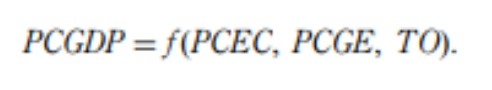
\includegraphics[scale=0.6]{electricity1.jpg}}
    \caption{Formulae 2.1}
\end{figure}
Where PCEC denotes the amount of power consumed per person (in kWh). The PCGDP stands for per capita GDP (constant 2010 in US dollar). PCGE (per capita government final consumption expenditure) and TO (trade of) are both in constant 2010 US dollars. \\
\begin{figure}[htbp]
    \centerline{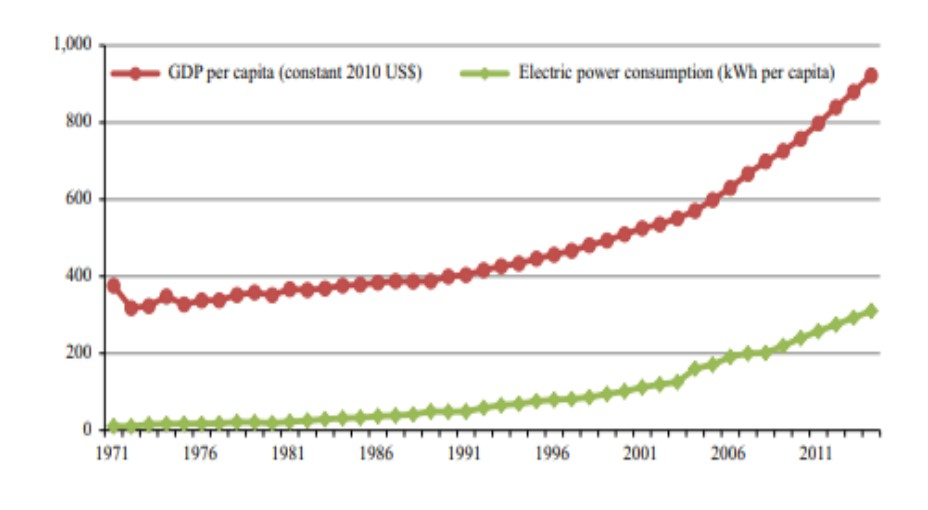
\includegraphics[scale=0.6]{electricity2.jpg}}
    \caption{A plot showing GDP and Electricity consumption}
\end{figure}
Once stationarity or cointegration is established, the econometric version of the aforementioned model linking to GDP and electricity
consumption was delivered as follows: $\alpha$  is the intercept, $\beta$1-$\beta$3 are the coefficients of exogenous variables
and $\varepsilon$  is the error term, all the variables stated in the functional form above are present. \\

\begin{figure}[htbp]
    \centerline{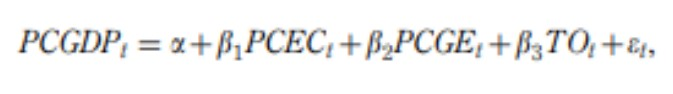
\includegraphics[scale=0.6]{electricity3.jpg}}
    \caption{Formulae 2.2}
\end{figure}
As a result, Strong evidence is being provided by both short-run and long-run coefficients that there is a significant positive relationship between electricity usage.
The bi-directional long-run causation between GDP and electricity consumption is further supported by a combined F-test. The robustness of their long run results was tested using three different estimators.
Their findings of positive electricity consumption-economic for the relationship between the development of financial activities and the economic growth in the country remain robust to all these three estimators .\\
Using this method, their overall study results suggest that the feedback hypothesis, which gives us the census that there is a two-way causal relationship between power consumed and GDP, exists both in the short-run and the long-run, showing that as Bangladesh's economy expands, electricity demand rises and vice versa.

\section{Dataset}
The "Our World in Data" proctors charting of how various different aspects of life impartially put together with GDP of a country. They are an organisation that provides research and data to mark progress against the world's largest problems.
\textbf{Sources:}\\
\begin{itemize}
    \item Our world in data,\textbf{\href{https://ourworldindata.org/}{GDP-electricity and -cereal yield}}
    \item Kaggle,\textbf{\href{https://www.kaggle.com/datasets/programmerrdai/financing-healthcare}{Healthcare financing Dataset}}
\end{itemize}
Since, there exists no one dataset that is feasible for this study a merged datset is need to be produced to calculate the various factors such as production, consumption and expenditure.
Kaggle is an other open-source dataset interceder that helps in finding out clean dataset \emph{(None of which were usable in this case, but it did help identify how such a dataset can be cleaned)}.
The datset that was finally made contained the following:
\begin{center}
    \begin{tabular}{ |c| }
        \hline
        Entity (Country name)       \\
        \hline
        Code                        \\
        \hline
        Year                        \\
        \hline
        Consumption (Electricity)   \\
        \hline
        Production (1.Meat)         \\
        Production (2.Cereal Yield) \\
        \hline
        Expenditure(Healthcare)     \\
        \hline
        GDP                         \\
        \hline
    \end{tabular}
\end{center}
\bigskip
\emph{The Code was the method of accesing a specific country or code together with the year acted as a unique identifier. The GDP is the exploratory variable. There are 2 different values for production due to data discrepancy.}
\section{Initial Insight (EDA)}
In order to understand the nature of the data, some of the attributes that were sorted for and mentioned above were analysed independently and compared on a global and nation-wise scale with 6 different countries for 4 different analysis, in order to find correlations and check inconsistency.
Visualizing such a dataset came up with intersting result which can be seen \textbf{\href{https://github.com/NeerajG03/Economic_Growth-Versus-Factors}{"here"}}.
The main visualization description that we attained is that meat consumption did not correlate highly with GDP.
This is due to the fact that consumption might vary on a per country basis.
Hence the change of consumption criteria was made to production of wheat, this still comes up short for many countries that are heavily reliant on meat as their primary source of nutrition.
Another observation from the data was that the correlation of GDP with accordance to healthcare expenditure and electricity consumption were usually high
\emph{(only usually in developing and developed country or countries with stable economy)}. This was especially seen in countries like Congo where the correlation was highly haphazardly correlated with almost all these factors.

\section{Acknowledgement}
From the members of this project we would like to extend our gratitude to Dr.Nagegowda who has helped us by providing us the opportunity for being able to create a study on such a topic, and guiding us along the way.
We would like to convey our appreciation towards the CSE department at PES University, for always inspiring us to conduct frequent research and inculcating a problem-solving discipline in us as well.
We would also like to acknowledge our assistant professors and the teaching assistants who have helped in the making and material of the course content and also the teaching assistants who have been constantly providing resources to practice the learnt concepts.
\begin{thebibliography}{00}
    \bibitem{b1} Ahmed Ibne Mahmood, Naznin Hossain, Sojib Bin Zaman,  Shuchita Sharmin Shakeel and Varshil Mehta,  \textbf{\href{https://jmrionline.com/jmri/article/view/72/86}{"An Association of Total Health Expenditure with GDP and Life Expectancy"}}, Vol 1 No 2 (2017) / AU7-AU12.
    \bibitem{b2} Mohammed Tareque and Sima Rani Dey, \textbf{\href{https://www.emerald.com/insight/content/doi/10.1108/JABES-04-2019-0029/full/pdf}{"Electricity consumption and GDP nexus in Bangladesh: a time series investigation"}}
    \bibitem{b3} Global Goals, \textbf{\href{https://www.globalgoals.org/goals/}{"The Global Goals of UN"}} \emph{Now changed from 8 goals to 17 goals}
    \bibitem{b4} Macroeconomics, \textbf{\href{https://www.worldbank.org/en/topic/macroeconomics/overview}{"Macroeconomics at a glance"}}
    \bibitem{b5} Massimiliano Marcellino, \textbf{\href{https://www.researchgate.net/profile/Niels-Haldrup/publication/228650389_A_comparison_of_time_series_models_for_forecasting_GDP_growth_and_inflation/links/0c96051b6b0d0e7951000000/A-comparison-of-time-series-models-for-forecasting-GDP-growth-and-inflation.pdf}{"A comparison of time series models for forecasting GDP growth and inflation"}}, April 2007 Curr. V3
\end{thebibliography}
\end{document}

